\documentclass[10pt]{scrartcl}
% \documentclass[10pt]{article}
\usepackage[T1]{fontenc}
\usepackage{amsmath,amsfonts,amssymb}
\usepackage{mathtools}
\usepackage{color,soul}
\usepackage{fullpage}
\usepackage{enumerate}
\usepackage{graphicx}
\usepackage[colorlinks=true,urlcolor=blue]{hyperref}
\usepackage{caption}
\usepackage{subcaption}
\usepackage{deluxetable}

\definecolor{Light}{gray}{.90}
\sethlcolor{Light}

\title{Multi-Sun Centroiding}
\author{Jeren Suzuki}
\date{Last Edited \today}

\begin{document}

\maketitle
\pagenumbering{Roman}
\tableofcontents
\clearpage
\pagenumbering{arabic}

\section{Introduction} % (fold)
\label{sec:introduction}
\hl{\texttt{beta}} is currently able to find the centers of these sun arrangements:

\begin{itemize}
    \item R1 \& R2
    \item R2 \& R3
    \item R1 \& R3
    \item R1 \& R2 \& R3
    \item R1 \& partial R2
    \item R1 \& partial R3
    \item R2 \& partial R3
    \item partial R1 \& R2
    \item partial R1 \& R3
    \item R1 \& partial R2 \& R3
    \item partial R1 \& R2 \& R3
    \item R1 \& partial R2 \& partial R3
    \item partial R1 \& partial R2 \& R3
    \item partial R1 \& R2 \& partial R3
\end{itemize}

This program will not be developed further bar bug-fixes I haven't noticed. \\
% section introduction (end)

\section{Partial Suns} % (fold)
\label{sec:partial_suns}

The current method to find the centers of any solar image is the following:

\begin{enumerate}
    \item Load Image
    \item Read parameters from pblock.txt
    \item Sort image and cut off top .1\% of pixels (top 1\% was actually too much)
    \item Smooth, take deriv, smooth again, take deriv again of sorted array, find peaks that correspond to difference solar regions and their thresholds
    \item Mask image above thresholds to find centers of every shape, regardless of partial or not
    \item Scan border of image looking for consecutive pixels above lowest threshold
    \item If more than 5 pixels in a row, marks x and y position and tags nearest solar center as ``partial''
    \item Crop remaining whole suns
    \item Extract 5 strips centered around cropped solar center for both X and Y direction
    \item Extract a pair of limb strips for each long strip
    \item Fit 2D polynomial to limb profile
    \item Mark position where fitted polynomail crosses threshold 
    \item Average midpoints of chords to find limb-fitted centers
\end{enumerate}

\begin{figure}[!ht]
    \centering
    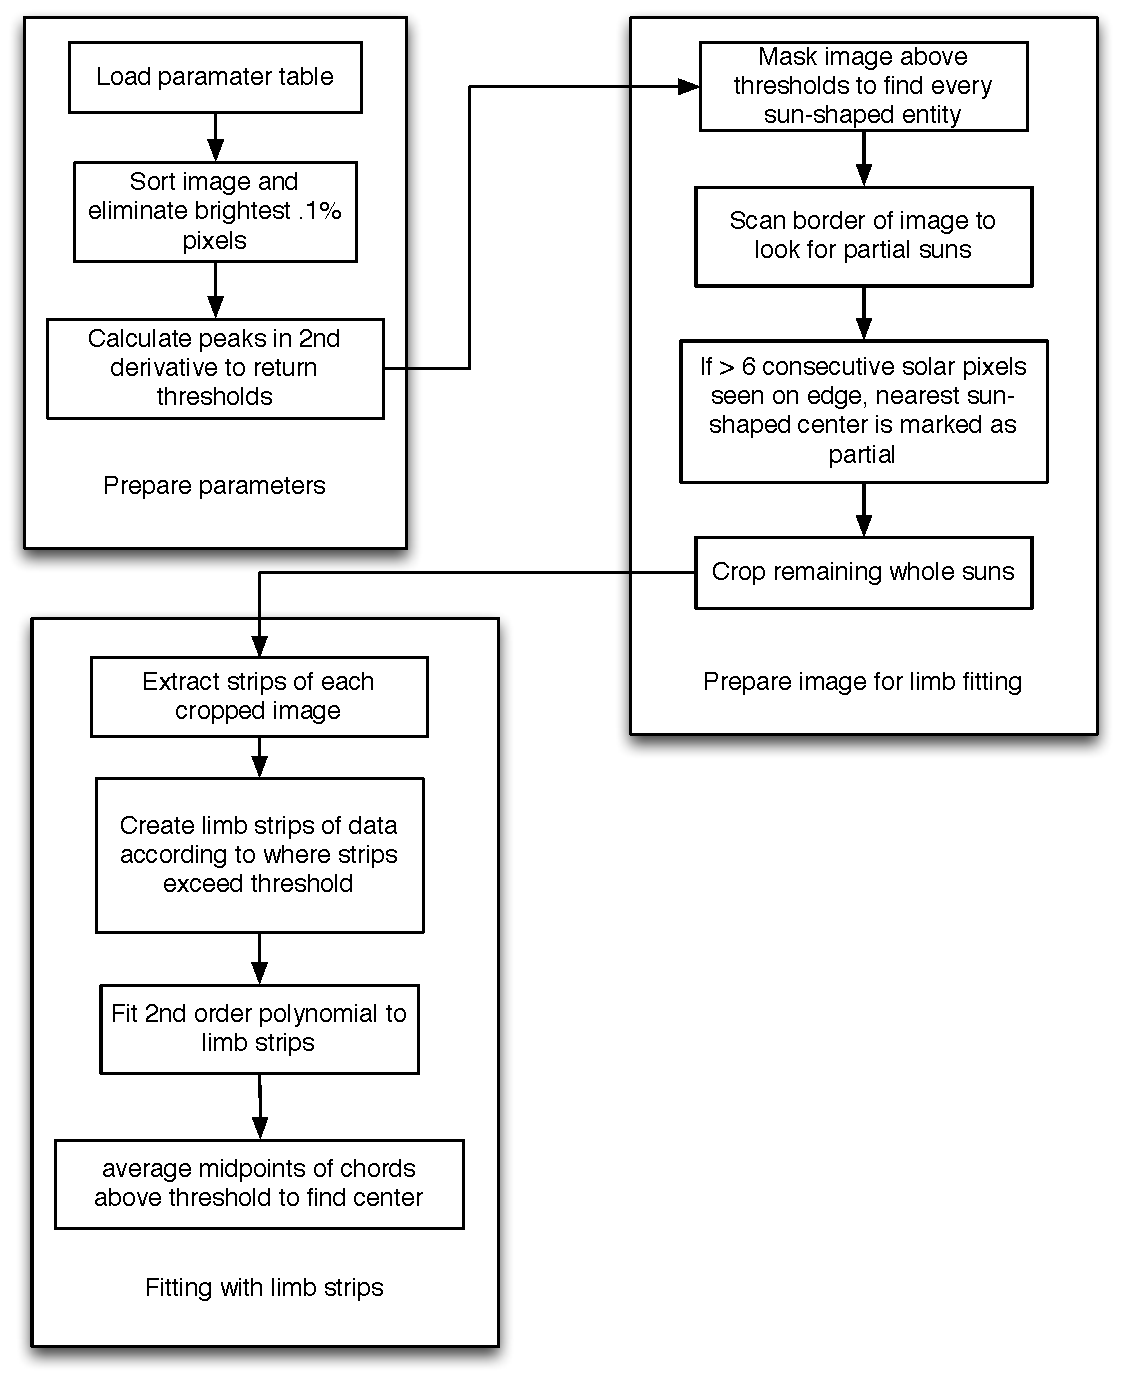
\includegraphics[width=.9\textwidth]{../plots_tables_images/beta_flowchart.pdf}    
\end{figure}


% section partial_suns (end)

\end{document}










